% FEEDBACK
%
% !TEX root = ../thesis-main.tex
%
\chapter{Feedback on lexical stress errors}
\label{chap:feedback}

%\cleanchapterquote{You can’t do better design with a computer, but you can speed up your work enormously.}{Wim Crouwel}{(Graphic designer and typographer)}

Since the focus of this thesis is on pronunciation training, not pronunciation assessment (see \cref{sec:capt:systems}), feedback on the errors diagnosed via the methods described in \cref{chap:diagnosis} is an important component of the prototype CAPT tool developed in this work. As mentioned in \cref{sec:capt:l2ed}, the particular importance of corrective feedback in pronunciation training is generally acknowledged,
%\citep{Neri2002,Dlaska2013}, 
though much remains to be learned about when and how feedback can be most effective. Therefore, an important contribution of this thesis is the creation of a feedback module for the lexical stress CAPT tool which offers a variety of possible feedback types, and a Graphical User Interface (GUI) allowing a researcher or instructor to easily switch between feedback types. The hope is that researchers can use this modular tool in in-vivo studies with language learners to compare the effects of various feedback types on the acquisition of L2 German prosody by L1 French speakers (or perhaps even speakers of other L1s); though it is outside the scope of the thesis to carry out 
such studies,
%in vivo studies with learners to determine which feedback types are most effective in which situations, 
the tool has been designed 
with this application in mind.
%to facilitate such studies going forward. 
Ultimately, once research has given us a better understanding of which feedback types are most effective in which situations, the modular feedback delivery system developed here could theoretically be embedded in a full-featured intelligent tutoring system, where models of the relevant learning contexts (such as  the objectives of the current exercise, or the student's past achievements and personal goals and preferences) could be used to automatically select the most useful feedback type to present to the learner, as mentioned in \cref{sec:intro:objectives} and illustrated in \cref{fig:hourglass-ITS,fig:feedback}.

This chapter presents the various options for the types of feedback that can be generated given a diagnosis of the learner's lexical stress realization, 
\TODO{\textit{rephrase:} guided by the notion that} to maximize its utility in future feedback research, the CAPT tool should offer as wide a variety of feedback options as possible, especially those offering types of feedback not commonly seen in existing CAPT systems. 
	\TODO{Some of these feedback options are visual \cref{sec:fb:visual}, some auditory \cref{sec:fb:auditory}, \TODO{\textit{reword:} and others constitute alternative feedback types} \cref{sec:fb:alternative}, as illustrated in \cref{fig:feedback}. }

%\textcite{Hattie2007} suggest that feedback in education should help the learner recognize their current learning goals (``Where am I going?''), assess their progress towards them (``How am I going?''), and identify next steps for achieving and moving beyond these goals (``Where to next?'').


%Feedback is important \citep{Neri2002}

%Since our focus is on pronunciation training and not just pronunciation assessment.



	\begin{figure}[htb]
		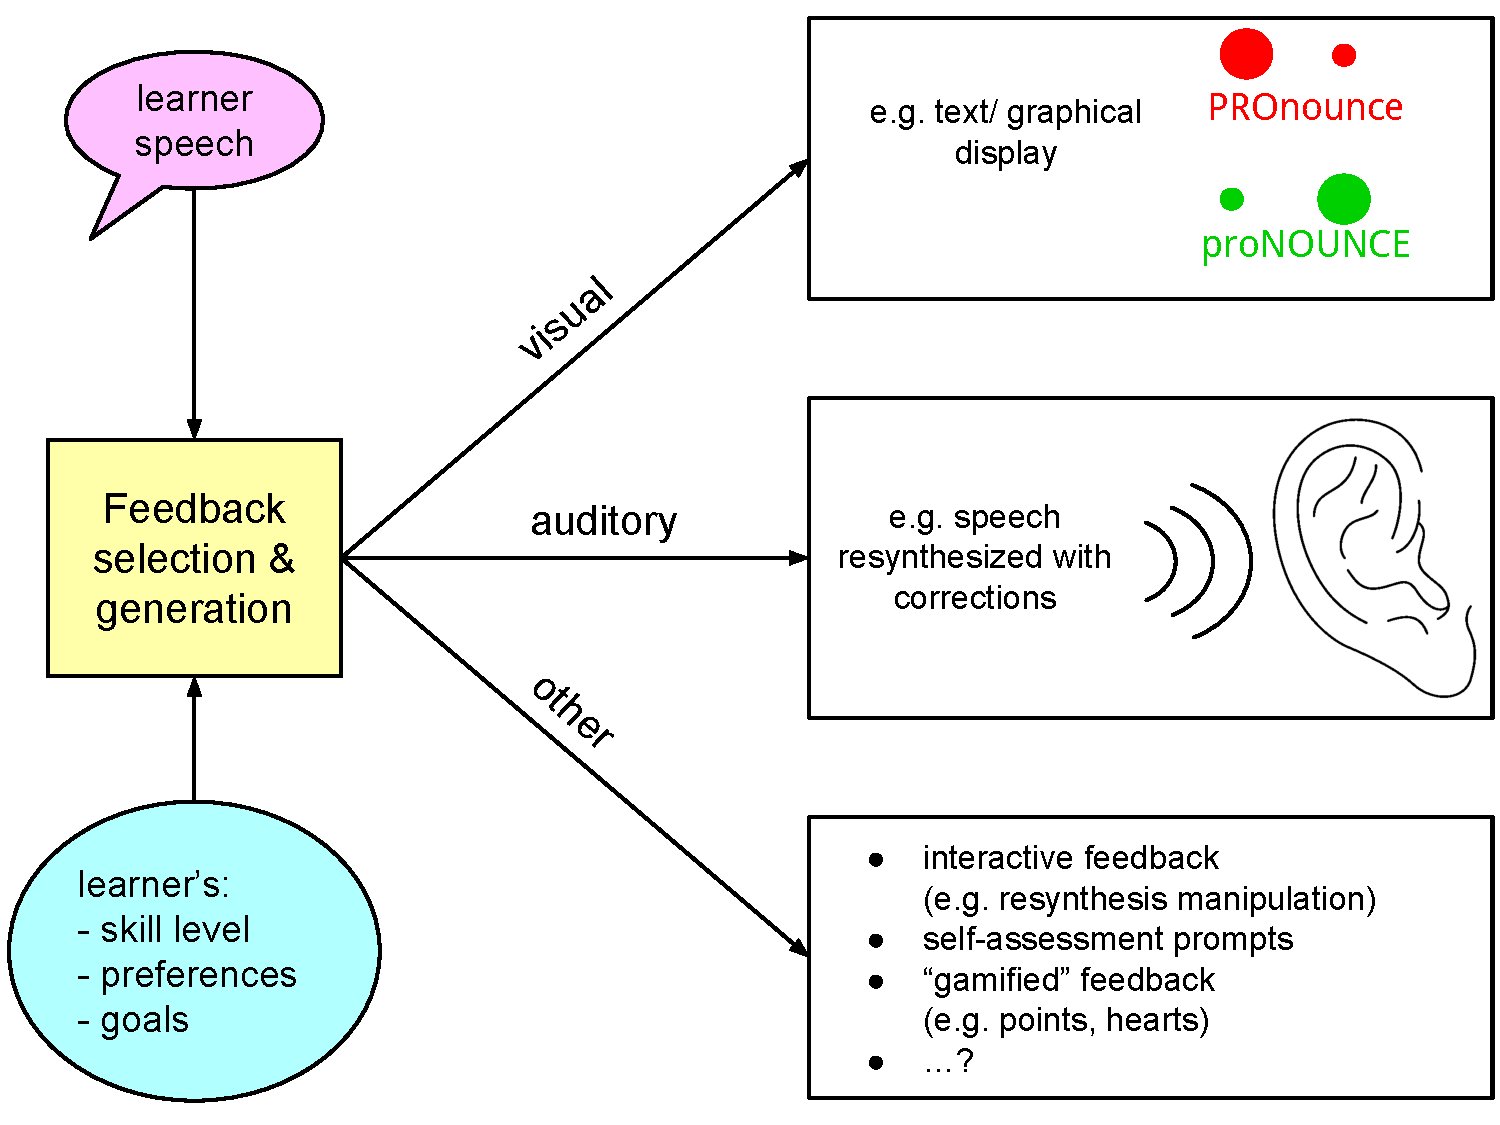
\includegraphics[width=\textwidth]{img/feedback}
		\caption{Delivery of prosody feedback in different modalities. \TODO{redo or remove}}
		\label{fig:feedback}
	\end{figure}

%\section{Related work}
%\label{sec:fb:related}
%
%	\cite{Sitaram2011}
%	\cite{Bonneau2011}
%	 	\citep{Hattie2007}




	\section{Implicit feedback}
	
		\TODO{Describe what implicit fb is}
	
		\subsection{Visual }
		
		Visual delivery of feedback on learner errors (or lack thereof) is a widely used technique in CAPT.
%	\subsection{Visualizations of the speech signal}
%	\label{sec:visual:visualizations}
	In many existing CAPT tools %such as Snoori \citep{Bonneau2011,Parole2013} and WinPitch LTL \citep{Martin2004}, 
	(e.g. \cite{Martin2004,Henry2007}),
the learner is presented with relatively direct visualizations of the speech signal, such as its waveform (oscillogram) and spectrogram, often with overlays highlighting perceptually relevant properties such as the pitch contour and durations of various parts of the utterance. 
	Indeed, this is the case in Jsnoori, as seen in \TODO{Jsnoori screenshot}.
	However, as \textcite{Neri2002} point out, waveforms and spectrograms are signal representations designed for speech researchers, not language learners, and the latter may have difficulty understanding these visualizations without the proper training. To research whether this conjecture holds, these direct visualizations must be compared with alternatives in user studies with learners; to this end, visual feedback in the lexical stress CAPT tool developed in this thesis project focuses on alternatives to direct signal visualizations, as described in this section.	
		
			\subsubsection{Graphical abstractions of prosody}
			\label{sec:implicit:visual:graphical}
			
			One type of alternative to direct visualizations of the speech signal is a more abstract graphical representation of the lexical stress pattern in the native reference speaker and/or the learner's speech. Classroom materials for pronunciation instruction sometimes represent lexical stress patterns using dots or other shapes, one for each syllable, whose relative sizes indicate each syllable's prominence in the word \citep{Hirschfeld1998}. By mapping the acoustic features of each syllable in the utterance(s) to graphical features (e.g. height, width) of a geometrical shape
			%-- e.g. using width to represent duration, height to represent F0, \TODO{and opacity to represent intensity} -- 
			it is possible to dynamically create a visual abstraction of the relevant properties of the learner's utterance as well as those of the reference utterance(s). This abstracted visual representation of prosody may be easier for the learner to interpret than the complex and possibly overwhelming signal visualizations more commonly used to give prosodic feedback in CAPT as mentioned in the previous section.
			
			\Cref{fig:rectangles} illustrates the display of such graphical abstractions in the prototype CAPT tool. Each syllable in an utterance is represented by a rectangle, the length of which corresponds to the duration of that syllable (as a percentage of the total word duration), the height of which represents the mean F0 in that syllable (normalized by dividing the absolute mean F0 for the syllable by the overall mean in the word), and the opacity of which corresponds to the mean intensity of that syllable (again normalized by dividing by the mean in the entire word). If the learner hovers their mouse over one of the rectangles, they are presented with the exact values for each of these features in a tooltip overlay, which can be seen as the small yellow box in the central area of \cref{fig:rectangles}.
			
				\begin{figure}
					\centering
					\caption[Feedback via graphical abstractions of prosody]{Screenshot of feedback via graphical abstractions of prosody}
					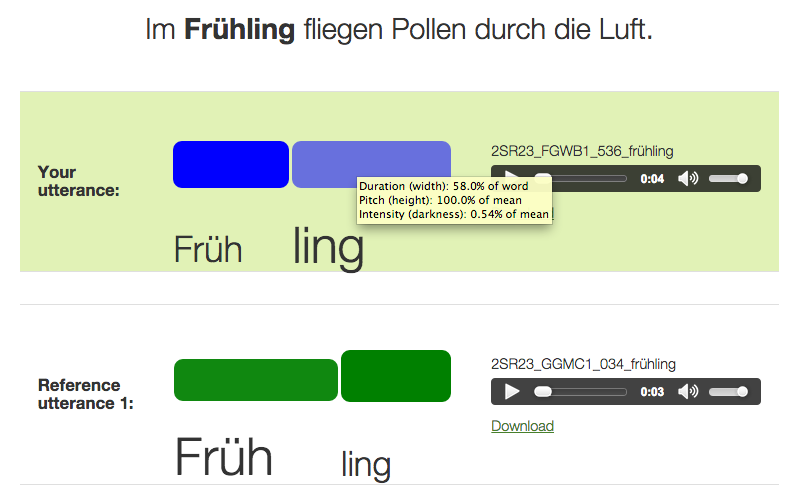
\includegraphics[width=\textwidth]{img/screenshots/rectanglesWithOpacity}
					\label{fig:rectangles}
				\end{figure}			
			
			In the prototype CAPT tool, the mappings between graphical properties (width, height, and opacity of the rectangle) and prosodic features (duration, F0, and intensity, respectively) are hard-wired. However, researchers using the system to experiment with different feedback methods should ideally be able to change the mapping or omit one of the features if necessary, so a more flexible feature-mapping mechanism would be a worthwhile improvement to the system (see \cref{sec:conclusion:future}).
			
			
			\subsubsection{Stylized text}
			\label{sec:implicit:visual:text}
			
			A related approach to the abstract graphical representations just described involves stylizing, or reshaping, the text of the word(s) pronounced  to match the prosodic features of the learner's utterance.
	This is essentially the approach used by the work \textcite{Sitaram2011}, who used text stylization to help visualize prosody in the Project LISTEN reading tutor (see \cref{sec:capt:listen}. 
	Such text stylization is also often used to convey canonical prosody in pronunciation instruction materials \citep{Behme-Gissel2005,Hirschfeld2007a}, e.g. by using larger text for the  stressed syllable than for the unstressed syllable(s) in a given word.
	Familiarity with this type of presentation might make feedback via stylized text easier for learners to comprehend, so text stylization was another form of implicit visual feedback implemented in the system, as illustrated in \cref{fig:textstylization}.
			
			
			\begin{figure}
			\centering
			\caption[Feedback on syllable duration via text stylization]{Screenshot of feedback on syllable duration via text stylization}
			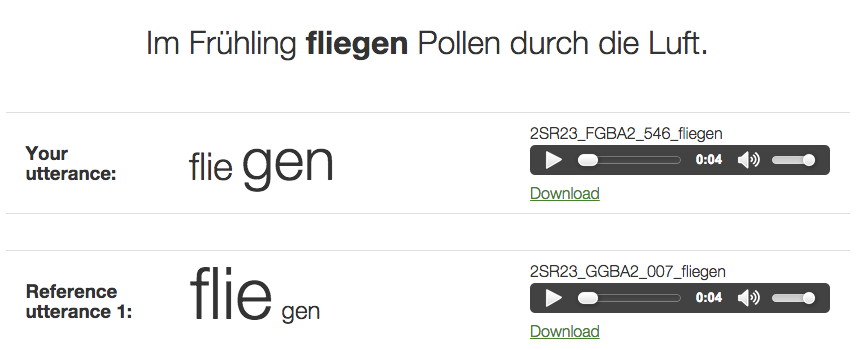
\includegraphics[width=\textwidth]{img/screenshots/textStylization}
			\label{fig:textstylization}
			\end{figure}
		
		
		When using geometric shapes to visualize prosody, different prosodic features can be conveyed simultaneously by mapping each to a different geometric property, as described in \cref{sec:implicit:visual:graphical} However, when dealing with text, visualizing multiple prosodic features at the same time is more difficult.
		First of all, noticing a clear difference between two syllables in terms of textual features such as height, font weight, or letter spacing is not as easy as comparing the height and width of two rectangles, given the inherent geometric variability of the different letters of the alphabet.
		Secondly, if text is stretched or skewed too dramatically, it becomes more difficult to read, which may be distracting for learners using the system. 
		
		
		Therefore, in the CAPT tool developed here, the text of a given syllable is stylized with a simple mapping between font size (as a multiple of the default size) and duration (as a fraction of the word duration). Duration was chosen as the prosodic feature to visualize based on its relative importance for the perception of lexical stress in German (see \cref{chap:diagnosis}). Font size was chosen as the textual feature to manipulate because it can be changed without distorting the text, i.e. without risking decreased legibility. Of course, other mappings between prosodic and textual features could be imagined, and once again the addition of other options than those currently implemented in the system could be worthwhile (see \cref{sec:conclusion:future}), though this might be less useful for text stylization than for  graphical visualizations, for the reasons mentioned in the previous paragraph.
		
			
			
		\subsection{Auditory}
		\label{sec:implicit:auditory}		
		\TODO{Is an intro necessary here? What should/can be said?}		
		
			\subsubsection{Student \& reference audio}
			\label{sec:implicit:auditory:basic}
			In foreign language classrooms, feedback on correct pronunciation is often given implicitly by
allowing the learner to listen to a native speaker's production of the target utterance and/or a recording of their own production. This type of implicit auditory feedback is perhaps the most simple feedback type to deliver, so the CAPT tool naturally offers learners the ability to listen to their own utterance as well as the reference utterance(s), and to download a wave file of any utterance for later reference if they so choose. Though learners may not always be able to detect errors in their pronunciation or possibilities for improvement from such implicit feedback alone, in conjunction with visual feedback of the types mentioned above this auditory feedback may help them improve their sensitivity to the stress patterns audible in the utterance(s). Therefore, as seen in \cref{fig:rectangles,fig:textstylization}, these audio recordings are always accessible alongside the visual (and other types of) feedback presented in the CAPT tool.
			
			\subsubsection{Resynthesized audio}
			\label{sec:implicit:auditory:resynth}
			
			As described in \cref{sec:capt:systems}, previous work on delivering lexical stress feedback 
has revealed that learners sometimes benefit from prosodically modified implicit auditory feedback, either in the form of a learner utterance  modified to reflect the ``correct'' prosody of a native reference utterance \citep{Bonneau2011}.
%TODO or a native utterance modified to place exaggerated emphasis on the stressed syllable \citep{Bissiri2006,Bissiri2009}.
			Thanks to the speech resynthesis capabilities of Jsnoori, this is another feedback option offered by the prototype CAPT tool.
			
			To modify the learner's utterance to match a reference utterance, Jsnoori uses the technique of Time Domain Pitch Synchronous Overlap and Add, or TD-PSOLA \citep{Moulines1990}. This technique uses the general strategy of creating a new, modified version of the original signal by using a windowing function to break the signal into a series of overlapping frames, where the spacing between those frames is pitch-synchronous, i.e. corresponds to the F0 period of (that part of) the signal. The duration of a region of the signal  (e.g. a vowel) can then be decreased or increased by removing or duplicating frames in that region while keeping the spacing between frames consistent, and  the perceived pitch of a region can be lowered or raised by increasing or decreasing the spacing between frames. The implementation of this signal-transformation technique in Jsnoori includes an improved method for detecting pitch marks in the original signal \citep{Laprie1998,Colotte2002}, as the accuracy of pitch marking is vitally important to the quality of resynthesis obtained via TD-PSOLA.
			
			To apply this technique in the context of prosody-oriented CAPT (see \cref{Henri2007,Bonneau2011}), the target prosody for that utterance is first established via analysis and comparison of F0 and duration in the learner and reference utterances, resulting in the computation of  target F0 contours and relative phone durations for (the relevant sections of) the learner's utterance. The learner's signal is then transformed to match the targets for F0 and duration by means of the removal/addition and re-spacing of frames, as described in the previous paragraph. The resulting signal maintains the individuality of the learner's voice, yet replaces their original ``incorrect'' prosody with the ``correct'' prosody of the reference speaker. 
			
			Like the Jsnoori software itself, the prototype CAPT tool offers the learner the opportunity to listen to this resynthesized utterance alongside their original utterance and that of the the native speaker. The hope is that by offering this this implicit auditory feedback as one of the many feedback types teachers/researchers can choose to present to the learner, the CAPT tool will facilitate further research into the use of this type of speech resynthesis for L2 language teaching.
			
			
	\section{Explicit feedback}
		\subsection{Skill bars}
		
		
		One way in which 
		the diagnosis of the learner's utterance in terms of duration, F0, and energy scores (calculated as
		%Jsnoori's diagnosis of a learner's utterance in terms of its timing (duration), pitch (F0), and energy (intensity), 
		described in \cref{sec:compare:single}) is made explicit to the learner is by means of graphical skill bars of the type often used in tutoring systems (e.g. \cite{Long2011,Long2013}).
		As illustrated in \cref{fig:skillbars:balanced,fig:skillbars:durpriority}, these bars provide explicit visual feedback for each ``skill'' (feature type) by displaying the score for that feature (as an integer out of 10, visible on the right hand side of the bar), as well as by graphically representing this score with both the length of the filled region of the bar (as a fraction of the total bar width corresponding to the score) and the color of that region (green for scores above 0.7, red for scores below 0.25, and yellow for intermediate scores).
		%
		 The bottom-most bar represents the overall score, computed as a weighted average of the three individual scores, using the weights assigned to each score by the researcher/teacher when configuring the diagnosis method \TODO{\cref{??}}.
		 
		  \Cref{fig:skillbars:balanced} illustrates a case where each of the three scores is given equal weighting, while \cref{fig:skillbars:durpriority} shows the same scores in the case where duration is prioritized over F0, which is in turn given a higher weight than intensity. \TODO{learner should be informed of the weighting - take new screenshot} Although the teacher or researcher setting up the exercise may (justifiably) choose to prioritize a feature, such as duration, in this way, one drawback of the skill bar visualization is that the equal size of the bars for each feature score seems to convey that all are equally important. Modifying the size of each bar based on the weight accorded to its feature may be a simple way to improve the effectiveness of this feedback type.% (see \cref{sec:conclusion:future})
		  
		  A potential problem with this feedback method relates to the fact, discussed in \cref{sec:compare:single}, that the scores output by Jsnoori's diagnostic tools are actually discrete, ordinal values, despite the use of numbers between 0 and 1 to represent these values. Therefore, the visual representation of these scores as if they belonged to a true interval or continuous variable is not necessarily justified, and this feedback may be somewhat confusing to the learner. It would be worthwhile to investigate this hypothesis through the type of in-vivo studies the CAPT tool has been designed to facilitate. 
		
%		\TODO{Skill bars may be misleading in that a) the scores are discrete, ordinal and not interval (see \cref{sec:compare:single:jsnoori}), b) displaying bars seems to accord equal importance to all three features, while we know that duration is most important}
		
			\begin{figure}
			\centering
			\caption[Skill bars as explicit feedback]{Screenshot of explicit feedback via skill bars, where all three skills (prosodic feature types) contribute equally to the overall score}
			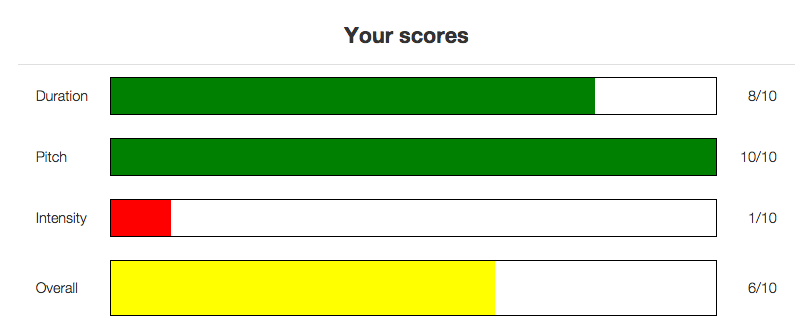
\includegraphics[width=\textwidth]{img/screenshots/skillBars-balanced-of10}
			\label{fig:skillbars:balanced}
			\end{figure}		
			
			\begin{figure}
			\centering
			\caption[Skill bars with unequal skill weights]{Screenshot of explicit feedback via skill bars, where duration contributes more than F0, which contributes more than intensity (60\%, 30\% and 10\% of overall score, respectively) \TODO{learner should be informed of the weighting - take new screenshot}}
			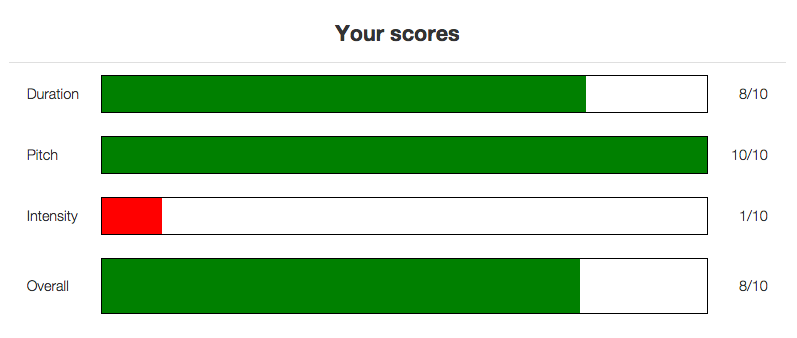
\includegraphics[width=\textwidth]{img/screenshots/skillBars-durPriority}
			\label{fig:skillbars:durpriority}
			\end{figure}	
		
		%\subsection{correct/incorrect/none classification}
		%TODO
		
		\subsection{Verbal feedback}
		
		Another way to explicitly deliver feedback on the learner's diagnosis is by verbalizing this diagnosis with one or more appropriate messages. 
		%
		If individual scores have been computed for the three prosodic feature types (duration, F0, and intensity) as described in \cref{sec:compare:single}, these are verbalized using the corresponding message from the set listed in \cref{tab:explicit:messages}.
		%
		If the learner's utterance has been diagnosed via classification and assigned one of the possible stress-accuracy labels (see \cref{sec:diag:classification}), that classification is verbalized with one of the following messages:
		\begin{itemize}
		\item{[correct]: ``You stressed the correct syllable. Great job!''}
		\item{[none]: ``It sounds like you pronounced both syllables with equal stress. Next time, try to use duration, pitch, and loudness to make the first syllable sound more important than the second syllable.''}
		\item{[incorrect]: ``It sounds like you stressed the incorrect syllable. Remember that the stress in <WORD> should be on the first syllable.''}
		\end{itemize}
		
		
		\begin{table}
			\centering
			\caption{Messages used to deliver explicit verbal feedback of feature-specific scores}
			\begin{tabular}{lll}
			\toprule
			Feature type & Score & Message \\
			\midrule 
			Duration (timing) & \TODO{} & \TODO{} \\
			F0 (pitch) & \TODO{} & \TODO{} \\
			Intensity (energy) & \TODO{} & \TODO{} \\

			\bottomrule
			\end{tabular}
			\label{tab:explicit:messages}
		\end{table}
		
		
		
		
	\section{Other types of feedback}
	\label{sec:fb:other}
	
		\subsection{Self-assessment}
		\label{sec:other:selfassess}
		
		\TODO{explain self-regulated learning, \citep{Long2011,Long2013}}
 
 	
 	In the prototype CAPT tool, learners can be encouraged to assess their own pronunciation by means of a short questionnaire optionally presented before any feedback has been delivered. This questionnaire, seen in \cref{fig:selfassess}, asks learners to listen to their utterance and that of the reference speaker(s) and assess whether they have placed stress on the correct syllable, whether stress is clearly realized in their utterance, and how they can improve their stress production going forward. The learner's responses to these questions are not evaluated in any way, but instead are \TODO{logged in the system} so that they can later reflect on their self-assessed progress and refer to their self-directed advice. 
 	
 	\TODO{It would be interesting to study whether requiring learners to complete this type of self-assessment activity has any influence on their self-regulated learning habits and, perhaps by extension, the improvement of their L2 prosody.}
 	
 	
 	\begin{figure}
		\centering
		\caption{Self-assessment questionnaire presented to learner before feedback delivery}
		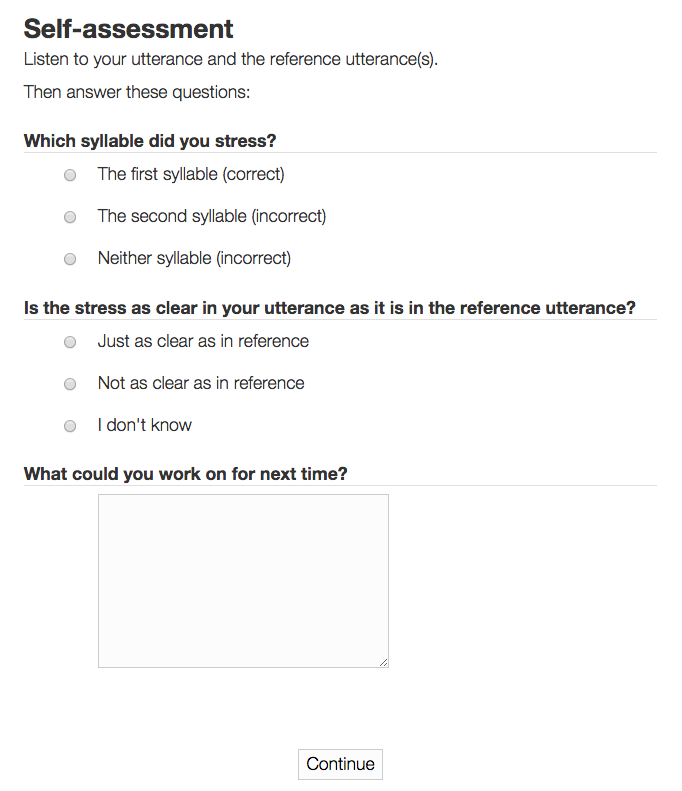
\includegraphics[width=.7\textwidth]{img/screenshots/selfAssessment}
		\label{fig:selfassess}
	\end{figure}
		
		
		
		
		\subsection{Metalinguistic feedback}
		\label{sec:other:meta}
	

	\TODO{Metalinguistic feedback, e.g. reminding learners %who have made an error 
of the stress rule(s) affecting the target utterance, could be delivered either visually (e.g. text displayed on the screen), auditorily (e.g. playback of an instructor's voice), or both. }


















%\section{Visual feedback}
%\label{sec:fb:visual}

%	Visual delivery of feedback on learner errors (or lack thereof) is a widely used technique in CAPT.
%%	\subsection{Visualizations of the speech signal}
%%	\label{sec:visual:visualizations}
%	In many existing CAPT tools %such as Snoori \citep{Bonneau2011,Parole2013} and WinPitch LTL \citep{Martin2004}, 
%	(e.g. \cite{Martin2004,Henry2007}),
%the learner is presented with relatively direct visualizations of the speech signal, such as its waveform (oscillogram) and spectrogram, often with overlays highlighting perceptually relevant properties such as the pitch contour and durations of various parts of the utterance. 
%	Indeed, this is the case in Jsnoori, as seen in \TODO{\cref{Jsnoori screenshot}}.
%	However, as \textcite{Neri2002} point out, waveforms and spectrograms are signal representations designed for speech researchers, not language learners, and the latter may have difficulty understanding these visualizations without the proper training. To research whether this conjecture holds, these direct visualizations must be compared with alternatives in user studies with learners; to this end, visual feedback in the lexical stress CAPT tool developed in this thesis project focuses on alternatives to direct signal visualizations, 
%	several types of which are presented in this section.
	
	
%	\subsection{Graphical representations of prosody}
%	\label{sec:visual:graphical}
%	


%	\TODO{\textit{DE-PROPOSAL-IZE} One type of alternative would be a more abstract graphical representation of the lexical stress pattern in the native reference speaker and/or the learner's speech. Classroom materials for pronunciation instruction sometimes represent lexical stress patterns using dots or other shapes, one for each syllable, whose relative sizes indicate each syllable's prominence in the word \citep{Hirschfeld1998}. This type of visualization would be relatively simple to implement, given that the reference or learner utterance can be classified into one of a set of stress patterns \citep{Kim2011,Shahin2012a}. It would also be possible to map the acoustic features of each syllable in the utterance(s) to graphical features of the representative shape, e.g. using size to represent duration, vertical position to represent F0, and darkness to represent intensity. 
	%MOVED TO FUTURE WORK
	%To facilitate studies on which mappings, if any, make this feedback useful to the learner, the researcher-facing GUI should offer control over the different possible mappings.}
	
%	\begin{figure}
%		\centering
%		\caption{Screenshot of feedback on syllable duration via graphical shapes \TODO{explain tooltip}}
%		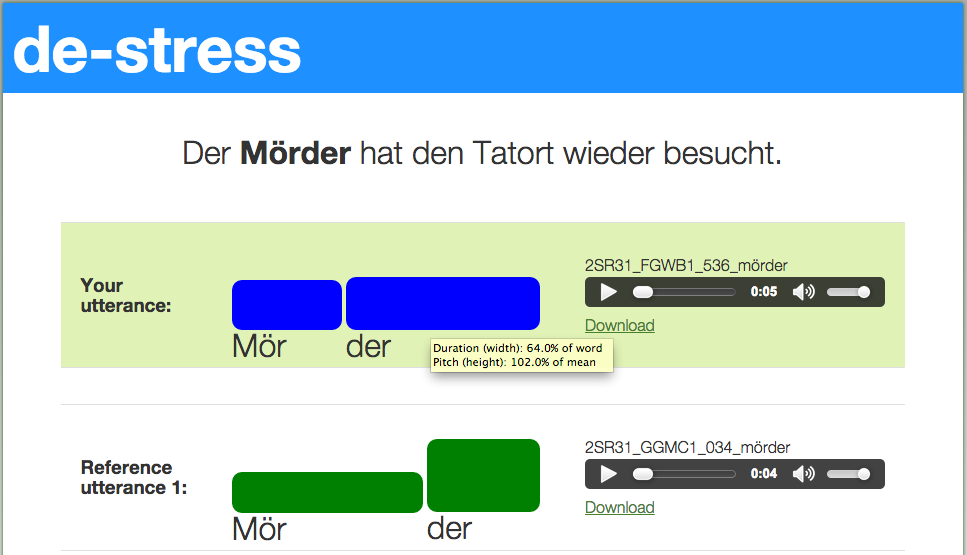
\includegraphics[width=\textwidth]{img/screenshots/rectangles}
%		\label{fig:visual:graphical}
%	\end{figure}
	
	
%	\subsection{Stylized text}
%	\label{sec:visual:text}
%	
%	In a related approach used by \textcite{Sitaram2011}, instead of displaying an abstract graphical representation of 	features of the learner's utterance, the text of the word(s) pronounced is stylized, or reshaped, to match these features.
%	%This is essentially the approach used by \textcite{Sitaram2011}, though they modify the text of each word instead of a more abstract visual representation. 
%	Such text stylization is also often used to convey canonical prosody in pronunciation instruction materials \citep{Behme-Gissel2005,Hirschfeld2007a}, 
%	and familiarity with this type of presentation might make feedback via stylized text easier for learners to comprehend; therefore,
%	including stylized text as a feedback option in the CAPT tool is a logical choice.
%	%so it would be logical for the CAPT tool to offer text stylization as a feedback option.
%	
%	\TODO{write up text stylization}	
%	
%	\begin{figure}
%	\centering
%	\caption[Feedback on syllable duration via text stylization]{Screenshot of feedback on syllable duration via text stylization  \TODO{crop out banner}}
%	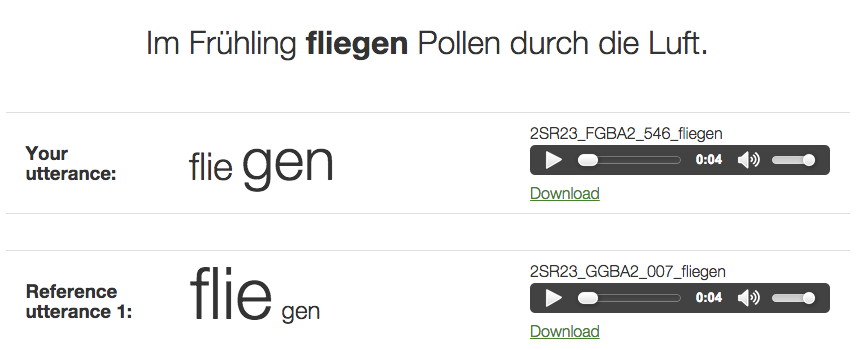
\includegraphics[width=\textwidth]{img/screenshots/textStylization}
%	\label{fig:visual:text}
%	\end{figure}
	
	
	%MOVED TO FUTURE WORK 
	%As with the shapes mentioned above, and following \textcite{Sitaram2011}, it would be interesting to explore the possible mappings between acoustic features and properties of the text of each syllable (e.g. size, weight, underlining/decoration, etc.), with these mappings controllable by the researcher via the GUI.

%Underlining \citep{Hirschfeld2007a}

%Bold + relative position of syllables \citep{Behme-Gissel2005}

%\subsection{Other}
%\label{sec:visual:other}


%\TODO{Given some visual representation of the learner's utterance, be it textual or more abstract, visual feedback should also be given on what the learner can do to improve their lexical stress realization. \textcite{Bonneau2011} deliver such feedback in the F0 dimension by displaying arrows which indicate whether the user should raise or lower the pitch of a given syllable to make their realization more like that of the reference speaker, and this is one option for the CAPT tool. Another might be the 
%MOVED TO FUTURE WORK
%use of animation to transform the visualization of the learner's (incorrectly realized) utterance into a corresponding visualization of the correct realization, e.g. by growing or shrinking the size of the dot or text for each syllable to visualize the desired change in duration, or showing it moving up or down to convey the desired change in pitch.}
	
	
%	Visualizations of the required articulators, such as those displayed in the Fluency pronunciation trainer \citep{Eskenazi2000}, may be helpful for correcting certain segmental errors, but are not likely of much use for correcting lexical stress, and will therefore not be implemented in the proposed tool.

%\TODO{	Implementation of at least one visual feedback type will be of high priority in this work. Stylized text and graphical representations will be explored first. If time allows, animation will be added to convey corrective feedback to the learner.
%}	
	
%\section{Auditory feedback}
%\label{sec:fb:auditory}
%
%%Some have speculated that auditory feedback may be more helpful than visual feedback in making learners more aware of lexical stress patterns \citep[p.~3]{Bissiri2009}, so it will be important to address both in the proposed CAPT tool.
%
%In foreign language classrooms, feedback on correct pronunciation is often given implicitly by
%%One strategy often used in classrooms is 
%%%implicit feedback, i.e. 
%allowing the learner to listen to a native speaker's production of the target utterance and/or a recording of their own production.
%% while there is no reason not to include the option for this type of implicit feedback in the CAPT tool, it will also be necessary to deliver explicit auditory feedback, as the latter may improve pronunciation more \citep{Dlaska2013} 
%	However, 
%%as described in \cref{sec:capt:systems} above, 
%previous work on delivering lexical stress feedback 
%(see \cref{sec:capt:systems}) 
%has revealed that learners seem to benefit more from prosodically modified implicit feedback, either in the form of a learner utterance  modified to reflect the ``correct'' prosody of a native reference utterance \citep{Bonneau2011}, or a native utterance modified to place exaggerated emphasis on the stressed syllable \citep{Bissiri2006,Bissiri2009}.
%	%In previous work on delivering %explicit 
%%feedback on lexical stress, as described in \cref{sec:capt:systems}, resynthesis of the learner's utterance has often been performed, where prosodic modifications are applied to make the utterance match the ``correct'' prosody of a reference utterance \citep{Bonneau2011,Bissiri2006,Bissiri2009}. 
%%	Another possibility to be explored follows \citeauthor{Bissiri2009} (\citeyear{Bissiri2006,Bissiri2009}), who found that presenting learners with native model utterances which had been modified to place exaggerated emphasis on the stressed syllable gave positive results. 
%	Therefore, these two types of modification may be implemented in the proposed CAPT tool's feedback module; the prosodic modification capabilities of the Jsnoori program \citep{Parole2013} will be used to transform the given utterance. 
%	If a more generalized model of the native prosody of a given word is developed (see \cref{sec:diag:compare}), it might also be possible to modify a reference (or learner) utterance to match this speaker-independent prosody.
	
%	At least one type of audio feedback type will be implemented in the CAPT tool, with the highest-priority option being prosodic modification of the learner's utterance to match a single, manually-selected reference utterance, following \textcite{Bonneau2011}; Jsnoori \citep{Parole2013} will be used to perform this modification.
%MOVED TO FUTURE WORK
% If a generalized lexical stress model is successfully integrated into the diagnostic module (see \cref{sec:diag:compare}), the next highest-priority task will be performing prosodic modification of the learner's utterance based on this model. Emphasizing stressed syllables in the native reference utterance(s) will be of lowest priority. 
	
	
 


%\citep{Jilka1998}?

%TODO replace
%	\subsection{Enhanced reference utterance}
%	\label{sec:auditory:enhanced}
%	
%TODO replace
%	\subsection{Resynthesized learner speech}
%	\label{sec:auditory:resynth}
	
	
	
%\section{Alternative feedback types}
%\label{sec:fb:alternative}

%Other options, which will only be explored if time allows, include (in order of priority) feedback encouraging self-assessment and self-correction, metalinguistic feedback, and interactivity. %TODO explain self-regulated learning
% 	Self-assessment and self-correction can be encouraged by presenting learners with targeted questionnaires before delivering diagnosis and feedback, e.g. asking learners to listen to their utterance and assess whether they have placed stress on the correct syllable, or 
% 	%asking them to listen to an incorrect production (theirs or another speaker's) and 
% 	asking how the speaker of an incorrect production could have realized stress properly (``By making the first syllable longer'', etc.). 
%	Metalinguistic feedback, e.g. reminding learners %who have made an error 
%of the stress rule(s) affecting the target utterance, could be delivered either visually (e.g. text displayed on the screen), auditorily (e.g. playback of an instructor's voice), or both. 
% 	Interactivity could be achieved by allowing learners to interact with the resynthesis component to modify the prosody of their utterance, as is done in WinPitch LTL \citep{Martin2004}. %TODO {Snoori too?} 
% 	By allowing researchers to easily control which of these feedback options to present to the learner, the tool could facilitate research into the effects of alternative feedback types such as these, which have not yet been adequately studied in CAPT.
 	
%	\subsection{Self-assessment}
%	\label{sec:alternative:selfassess}
%	
%	\TODO{}
% 	
% 	
% 	\begin{figure}
%		\centering
%		\caption{Self-assessment questionnaire presented to learner before feedback delivery}
%		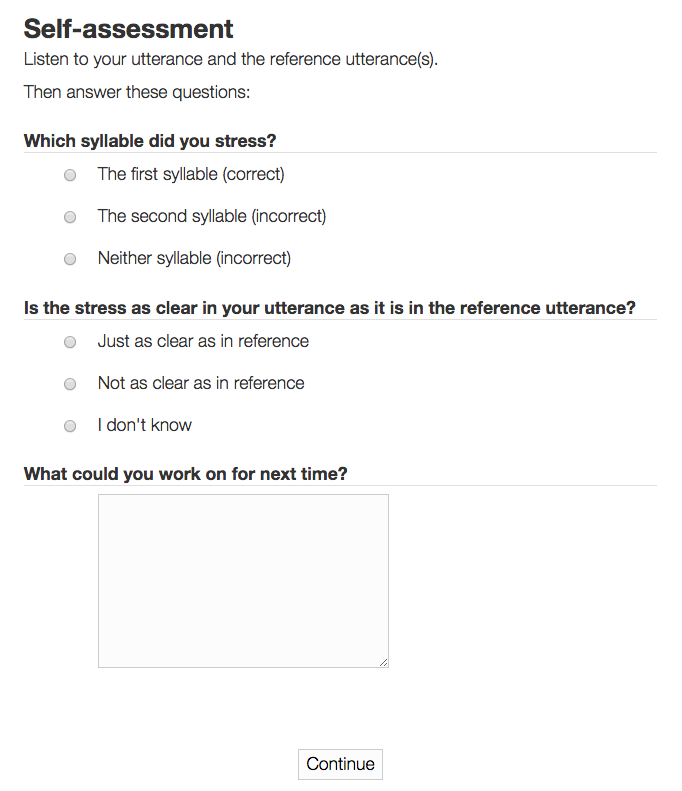
\includegraphics[width=.7\textwidth]{img/screenshots/selfAssessment}
%		\label{fig:visual:selfassess}
%	\end{figure}
% 

%	\subsection{Metalinguistic feedback}
%	\label{sec:alternative:metaling}
%	
%	\subsection{Interactive feedback}
%	\label{sec:alternative:interactive}
%	
%	\subsection{Implicit feedback}
%	\label{sec:alternative:implicit}


\section{\TODO{Controlling feedback methods in the system}}
\label{sec:fb:system}
\TODO{}

\section{Summary}
\label{sec:fb:summary}
\TODO{}